\documentclass[11pt]{article}
\usepackage{../cs70,latexsym,epsf}
\lecture{14}
\def\title{Note \the\lecturenumber}
\usepackage{tikz}
\usetikzlibrary[graphs]
\usetikzlibrary{matrix}
\usetikzlibrary{shapes,arrows,chains,positioning}
\usepgflibrary{arrows} % LATEX and plain TEX and pure pgf
\usepgflibrary[arrows] % ConTEXt and pure pgf
\usepgflibrary[plotmarks] % ConTEXt and pure pgf
\usetikzlibrary{arrows} % LATEX and plain TEX when

\usetikzlibrary{decorations,decorations.pathmorphing,decorations.markings}


%%% Alistair's Macros
\makeatletter
\def\eqalign#1{\,\vcenter{\openup\jot\m@th
  \ialign{\strut\hfil${##}$&${{}##}$\hfil
      \crcr#1\crcr}}\,}
\def\eqalignno#1{\displ@y \tabskip\@centering
  \halign to\displaywidth{\hfil${##}$\tabskip\z@skip
    &${{}##}$\hfil\tabskip\@centering
    &\llap{$##$}\tabskip\z@skip\crcr
    #1\crcr}}
\makeatother
\def\third{{\textstyle{1\over 3}}}
\def\half{{\textstyle{1\over 2}}}
\def\ul#1{\underline{#1}}
\def\VarOmega{\mathchar"10A }
\def\varOmega{\mathchar"10A }
\newenvironment{proposition}{\par\global\advance\theoremnumber by 1
{\bf Proposition \the\lecturenumber.\the\theoremnumber}:
\begingroup\em}%
{\endgroup}
%%% End Alistair's Macros

\newcounter{thm}
\addtocounter{thm}{\the\lecturenumber}
\newtheorem{theorem}{Theorem}[thm]
\newtheorem{definition}{Definition}[thm]


\begin{document}
\maketitle

\section*{Introduction}
One of the key properties of coin flips is independence: if you flip a fair 
coin ten times and get ten T's, this does not make it more likely that the 
next coin flip will be H's. It still has exactly $50\%$ chance of being H's. 

By contrast, suppose while dealing cards, the first ten cards are all red
(hearts or diamonds). What is the chance that the next card is red? This 
is easy: we started with exactly $26$ red cards and $26$ black cards. 
But after dealing the first ten cards we know that the deck has $16$ red
cards and $26$ black cards. So the chance that the next card is red is 
$\frac{16}{42}$. So unlike the case of coin flips, now the chance of 
drawing a red card is no longer independent of the previous card that
was dealt. This is the phenomenon we will explore in this note on conditional 
probability. 

\section*{Conditional Probability}

Let's consider an example with a smaller sample space.  
Suppose we toss $m=3$ balls into $n=3$
bins; this is a uniform sample space with $3^3=27$ points.  
We already know that the probability the first bin is empty
is $(1-{1\over 3})^3=({2\over 3})^3={8\over{27}}$.  What is the
probability of this event {\it given that\/} the second bin is
empty?  Call these events $A,B$ respectively. In the language of conditional
probability we wish to compute the probability $P[A\vert B]$, which 
we read to say probability of $A$ given $B$. 

How should we compute $\Pr[A\vert B]$?  Well, since event $B$ 
is guaranteed to happen, we need to look not at the whole sample
space~$\VarOmega$, but at the smaller sample space consisting 
only of the sample points in~$B$.  In terms of the picture below, we are no longer
looking at the large oval, but only the oval labeled $B$: 

%% \begin{center}
%% 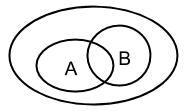
\includegraphics[scale = .70]{conditional.png}
%% \end{center}

\begin{center}
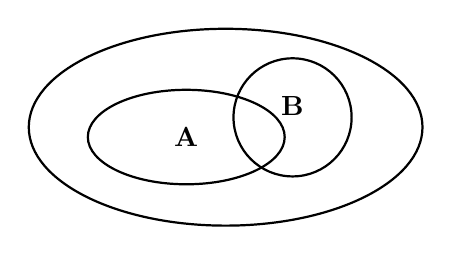
\begin{tikzpicture}[scale=.5]

\draw[thick]  {(0,0) ellipse (5cm and 2.5cm)};
\draw[thick]  {(-1,-.25) ellipse (2.5cm and 1.2cm)};
\draw[thick]  {(1.7,.25) ellipse (1.5cm and 1.5cm)};


\node at (-1,-.25) {\bf A};
\node at (1.7,.55) {\bf B};
\end{tikzpicture}
\end{center}

What should the probabilities
of these sample points be?  If they all simply inherit their
probabilities from~$\VarOmega$, then the sum of these probabilities
will be $\sum_{\omega\in B}\Pr[\omega]=\Pr[B]$, which in general
is less than~1.  So we need to {\it scale\/} the probability
of each sample point by~$1\over{\Pr[B]}$.  I.e., for each sample
point $\omega\in B$, the new probability becomes $$
   \Pr[\omega\vert B]={{\Pr[\omega]}\over{\Pr[B]}}.  $$
   Now it is clear how to compute $\Pr[A\vert B]$: namely, we just
sum up these scaled probabilities over all sample points that
lie in both~$A$ and~$B$:  $$
   \Pr[A\vert B] = \sum_{\omega\in A\cap B} \Pr[\omega\vert B]
                 = \sum_{\omega\in A\cap B} {{\Pr[\omega]\over{\Pr[B]}}}
                 = {{\Pr[A\cap B]}\over{\Pr[B]}}.  $$

\begin{definition}[Conditional Probability]\label{defcp}
For events $A,B$ in the same probability space, such that 
$\Pr[B]>0$, the \ul{conditional probability of~$A$ given~$B$}
is $$
   \Pr[A\vert B] = {{\Pr[A\cap B]}\over{\Pr[B]}}.  $$
\end{definition}
   
Returning to our example, to compute $\Pr[A\vert B]$
we need to figure out $\Pr[A\cap B]$.  But $A\cap B$ is the event 
that both the first two bins are empty, i.e., all three balls fall in the
third bin.  So $\Pr[A\cap B]={1\over{27}}$ (why?).  Therefore, $$
   \Pr[A\vert B] = {{\Pr[A\cap B]}\over{\Pr[B]}} = {{1/27}\over{8/27}} = {1\over 8}.
 $$
Not surprisingly, $1\over 8$ is quite a bit less than $8\over{27}$: 
knowing that bin~2 is empty makes it significantly less likely that
bin~1 will be empty.
 
 \subsection*{Example: Card Dealing}

Let's apply the ideas discussed above to compute the probability 
that, when dealing 2 cards and the first card is known to be an ace,
the second card is also an ace. Let $B$ be the event that the first
card is an ace, and let $A$ be the event that the second card is an ace. 
Note that $P[A] = P[B] = {1\over 13}$. 

To compute $\Pr[A\vert B]$, we need to figure out $\Pr[A\cap B]$.  
This is the probability that both cards are aces. Note that there are 
$52\cdot 51$ sample points in the sample space, since each sample 
point is a sequence of two cards. A sample point is in $A\cap B$ if both
cards are aces. This can happen in $4\cdot 3 = 12$ ways. 

Since each sample point is equally likely, $\Pr[A\cap B] = \frac{12}{52\cdot 51}$. 
The probability of event $B$, drawing an ace in the first trial, is $\frac{4}{52}$. 
Therefore, $$\Pr[A\vert B] = {{\Pr[A\cap B]}\over{\Pr[B]}} = {3\over 51}.
 $$
 
 Note that this says that if the first card is an ace, it makes it less likely that
 the second card is also an ace. 
 
 \section*{Bayesian Inference}
 Now that we've introduced the notion of conditional probability, we can see
 how it is used in real world settings. Conditional probability is at the heart
 of a subject called {\em
Bayesian inference}, used extensively in fields such as machine
learning, communications and signal processing. Bayesian inference
is a way to {\em update knowledge} after making an
observation. For example, we may have an estimate of the probability
of a given event $A$. After event $B$ occurs, we can update this estimate to $\Pr[A|B]$. 
In this interpretation, $\Pr [A]$ can be thought of as
a {\em prior} probability: our assessment of the likelihood of an
event of interest $A$  {\em before} making an observation. It
reflects our prior knowledge. $\Pr [A|B]$ can be interpreted as the
{\em posterior} probability of $A$ after the observation. It
reflects our new knowledge.

Here is an example of where we can apply such a technique. 
A pharmaceutical company is marketing a new test for a certain
medical disorder.  According to clinical trials, the test has
the following properties:
\begin{enumerate}
\item When applied to an affected person, the test comes up
positive in 90\% of cases, and negative in 10\% (these are
called ``false negatives'').
\item When applied to a healthy person, the test comes up
negative in 80\% of cases, and positive in 20\% (these are
called ``false positives'').
\end{enumerate}
Suppose that the incidence of the disorder in the US population
is~5\%; this is our prior knowledge. When a random person is tested and the test comes up
positive, how can we update this probability? (Note that this is presumably {\it not\/} the
same as the simple probability that a random person has the
disorder, which is just~$1\over{20}$.)  The implicit probability
space here is the entire US population with uniform probabilities.

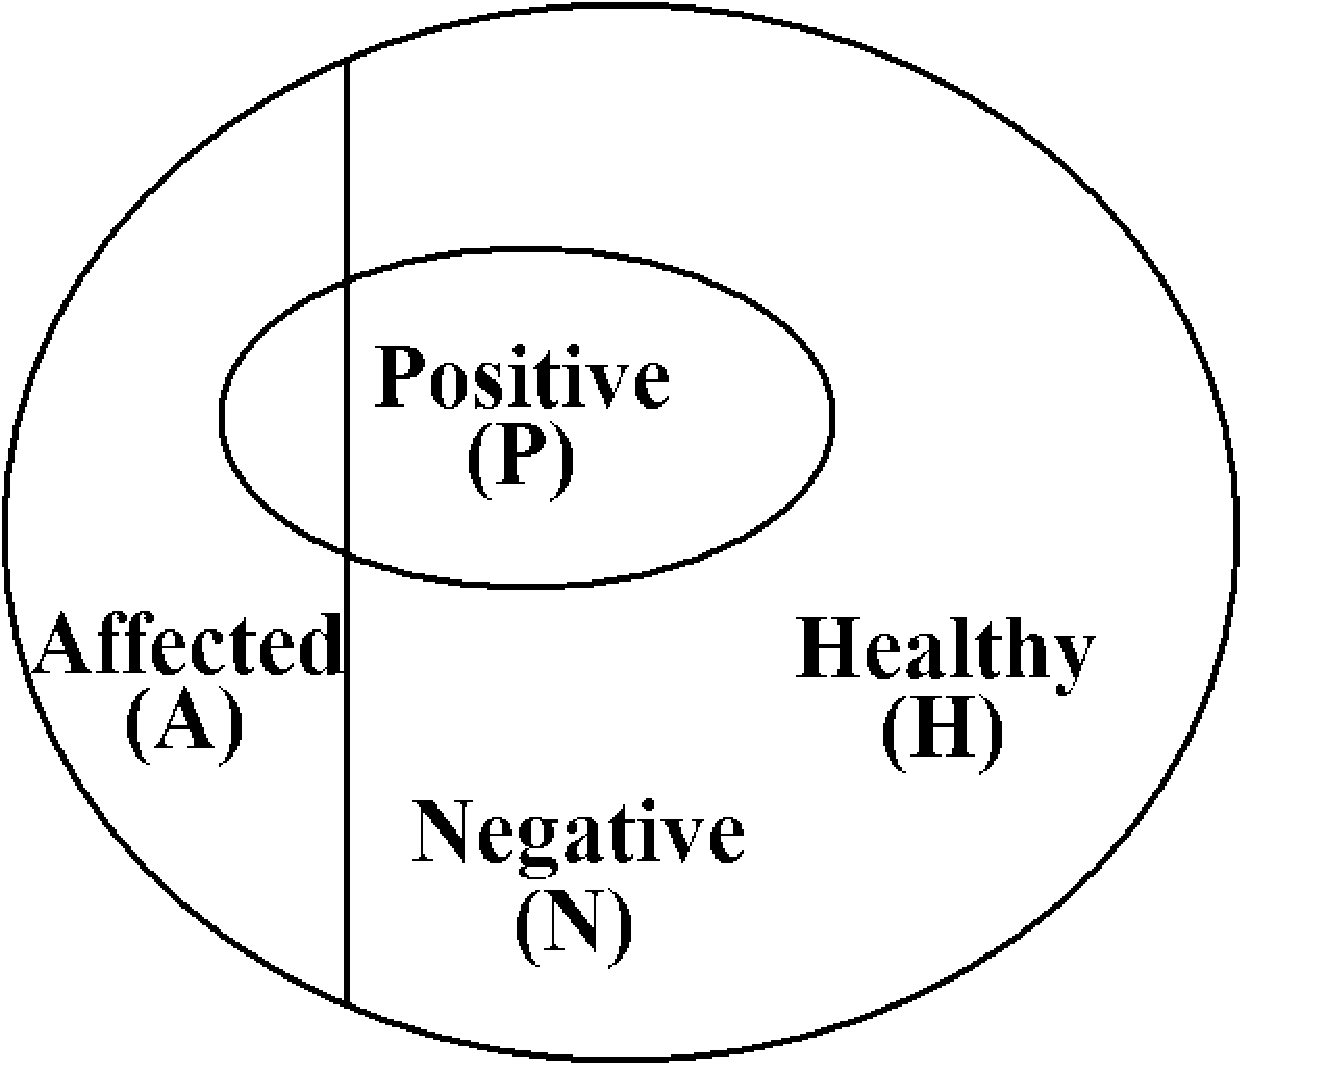
\includegraphics[bb = -400 0 0 520, scale = 0.22]{pharmacy.pdf}

The sample space here
consists of all people in the US --- denote their number by~$N$
(so $N\approx 250$ million). Let $A$ be the event that a person chosen
at random is affected, and $B$ be the event that a person chosen at random
tests positive. Now we can rewrite the information above:
\begin{itemize}

\item $\Pr [A] = 0.05$, ($5\%$ of the U.S. population is affected)

\item $\Pr [B|A] = 0.9$ ($90\%$ of the affected people test positive)

\item $\Pr [B|\overline{A}] =0.2$ ($20\%$ of healthy people test positive)

\end{itemize}

We want to calculate $\Pr [A|B]$. We can proceed as follows:

\begin{equation}
\label{eq:bayes}
 \Pr [A|B] = \frac{\Pr [A\cap B]}{\Pr [B]} = \frac{\Pr [B|A]\Pr [A]}{\Pr [B]}
 \end{equation}

 We obtained the second equality above by applying the definition 
 of conditional probability:
 $$
 \Pr[B|A] = \frac{\Pr[A\cap B]}{\Pr[A]}
 $$
 
 Now we need to compute $\Pr[B]$. This is the probability that
 a random person tests positive. To compute this, we can sum two values:
 the probability that a healthy person tests positive, $\Pr[\bar{A}\cap B]$ and the
 probability that an affected person tests positive, $\Pr[A\cap B]$. We can sum because
 the events $\bar{A}\cap B$ and $A\cap B$ do not intersect:
 
%% \begin{center}
%% 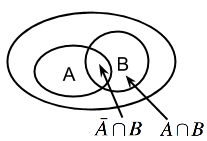
\includegraphics[scale = .70]{sum.png}
%% \end{center}

\begin{center}
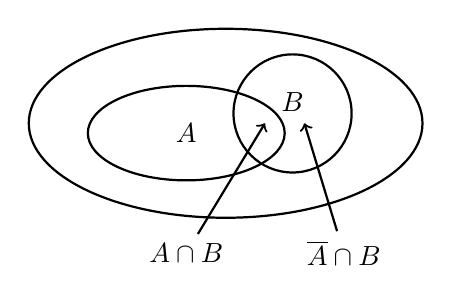
\begin{tikzpicture}[scale=.5]

\draw[thick]  {(0,0) ellipse (5cm and 2.4cm)};
\draw[thick]  {(-1,-.25) ellipse (2.5cm and 1.2cm)};
\draw[thick]  {(1.7,.25) ellipse (1.5cm and 1.5cm)};


\node at (-1,-.25) {\bf $A$};
\node at (1.7,.55) {\bf $B$};

\node(int) at (-1,-3.3) {\bf ${A} \cap B$};
\node(intn) at (3,-3.3) {\bf $\overline{A} \cap B$};

\draw[->,thick] (int) -- (1,0);
\draw[->,thick] (intn) -- (2,0);

\end{tikzpicture}
\end{center}
 
By again applying the definition of conditional probability we have:
 \begin{equation}
\label{eq:total}
 \Pr [B] = \Pr [A \cap B] + \Pr [\overline{A} \cap B] = \Pr [B|A]\Pr [A] +
\Pr [B|\overline{A}] (1-\Pr [A])
 \end{equation}
 
Combining equations (\ref{eq:bayes}) and (\ref{eq:total}),  we have
expressed $\Pr [A|B]$ in terms of $\Pr [A], \Pr [B|A] $ and $\Pr
[B|\overline{A}]$:

\begin{equation}
\label{eq:update}
 \Pr [A|B] = \frac{\Pr [B|A] \Pr [A]}{\Pr [B|A]\Pr [A] +
\Pr [B|\overline{A}] (1-\Pr [A])}
 \end{equation}
 
 By plugging in the values written above, we obtain $\Pr[A|B] = \frac{9}{47}\approx .19$. 

Equation (\ref{eq:update}) is useful for many inference problems. We are given
$\Pr [A]$, which is the (unconditional) probability that the event
of interest $A$ happens. We are given $\Pr [B|A]$ and $\Pr
[B|\overline{A}]$, which quantify how noisy the observation is. (If
$\Pr [B|A] =1$ and $\Pr [B|\overline{A}] = 0$, for example, the
observation is completely noiseless.) Now we want to calculate $\Pr
[A|B]$, the probability that the event of interest happens given we
made the observation. Equation (\ref{eq:update}) allows us to do
just that.\\\\


Of course, equations (\ref{eq:bayes}), (\ref{eq:total}) and
(\ref{eq:update}) are derived from the basic axioms of probability
and the definition of conditional probability, and are therefore
true with or without the above Bayesian inference interpretation.
However, this interpretation is very useful when we apply
probability theory to study inference problems.

\section*{Bayes' Rule and Total Probability Rule}

Equations (\ref{eq:bayes}) and (\ref{eq:total}) are very useful in
their own right. The first is called {\bf Bayes' Rule} and the
second is called the {\bf Total Probability Rule}. Bayes' rule is
useful when one wants to calculate $\Pr [A|B]$ but one is given $\Pr
[B|A]$ instead, i.e. it allows us to "flip" things around. 

The Total
Probability rule is an application of the strategy of "dividing into
cases" .There are two
possibilities: either an event $A$ happens or $A$ does not happen. 
If $A$ happens the probability that $B$ happens is $\Pr [B|A]$. If
$A$ does not happen, the probability that $B$ happens is $\Pr
[B|\overline{A}]$. If we know or can easily calculate these two
probabilities and also $\Pr [A]$, then the total probability rule
yields the probability of event $B$.

\subsection*{Example: Tennis Match}
You are about to play a tennis match against a randomly
chosen opponent and you wish to calculate your probability of winning.
You know your opponent will be one of two people, $X$ or $Y$. If person $X$ is chosen,
you will win with probability .7. If person $Y$ is chosen, you will win with probability .3. 
Your opponent is chosen by flipping a coin with bias .6 in favor of $X$. 

Let's first determine which events we are interested in. Let $A$ be the event that you win.
Let $B_1$ be the event that person $X$ is chosen, and let $B_2$ be the event that person $Y$ is chosen.
We wish to calculate $\Pr[A]$. Here is what we know so far: 

\begin{itemize}

\item $\Pr [A|B_1] = 0.7$, (if person $X$ is chosen, you win with probability .7)

\item $\Pr [A|B_2] = 0.3$ (if person $Y$ is chosen, you win with probability .3)

\item $\Pr [B_1] =0.6$ (person $X$ is chosen with probability .6)

\item $\Pr[B_2] =0.4$ (person $Y$ is chosen with probability .4)

\end{itemize}

By using the Total Probability rule, we have:
$$
\Pr[A] = \Pr[A|B_1]\Pr[B_1] + \Pr[A|B_2]\Pr[B_2]. 
$$

Now we can simply plug in the known values above to obtain $\Pr[A]$:
$$
\Pr[A] = .7\times.6 + .3\times .4 = .54
$$

\subsection*{Example: Balls and Bins}
Imagine we have two bins containing black and white balls, and further suppose that we wanted
to know what is the chance that we picked Bin 1 given that we picked a white ball, i.e., $\Pr[$Bin $1|$ \setlength{\unitlength}{.1in}
\begin{picture}(.5,1)(0,0)
\linethickness{1pt}
\put(-.25,.4){\circle{1}}
\end{picture}$]$.  Assume that we are unbiased when choosing a bin so that each bin is chosen with probability $\frac{1}{2}$.

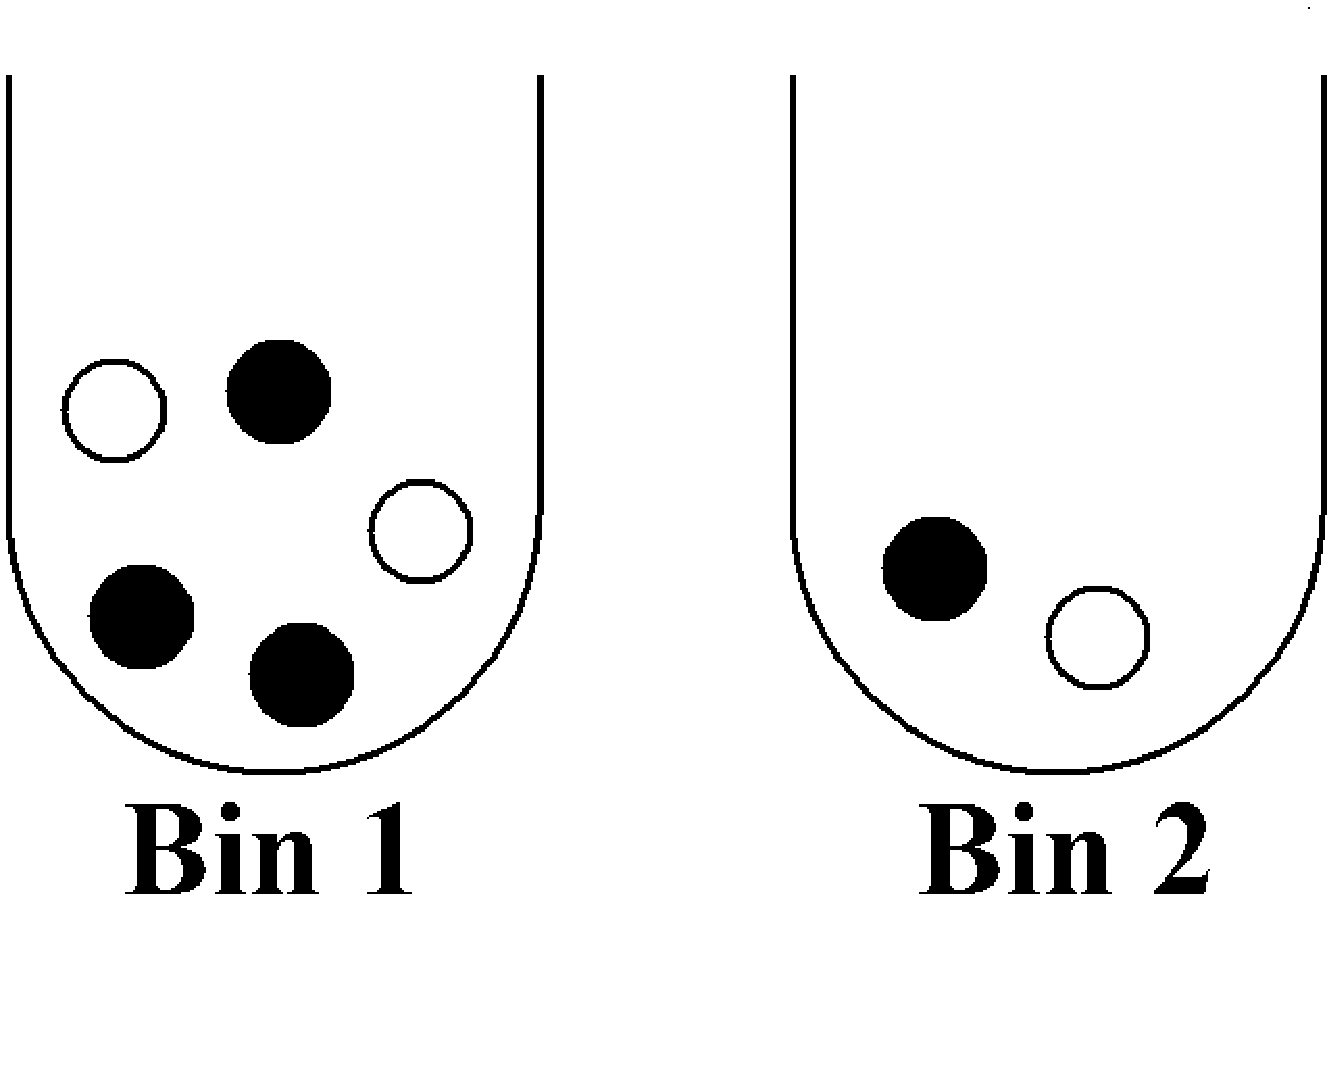
\includegraphics[bb = -580 60 100 620, scale = 0.24]{bins.pdf}

A wrong approach is to say that the answer is clearly $\frac{2}{3}$, since we know there are a total of three white balls, two of which are in bin 1.  However, this picture is misleading because the bins
have equal ``weight".  Instead, what we should do is appropriately scale each sample
point as the following picture shows:

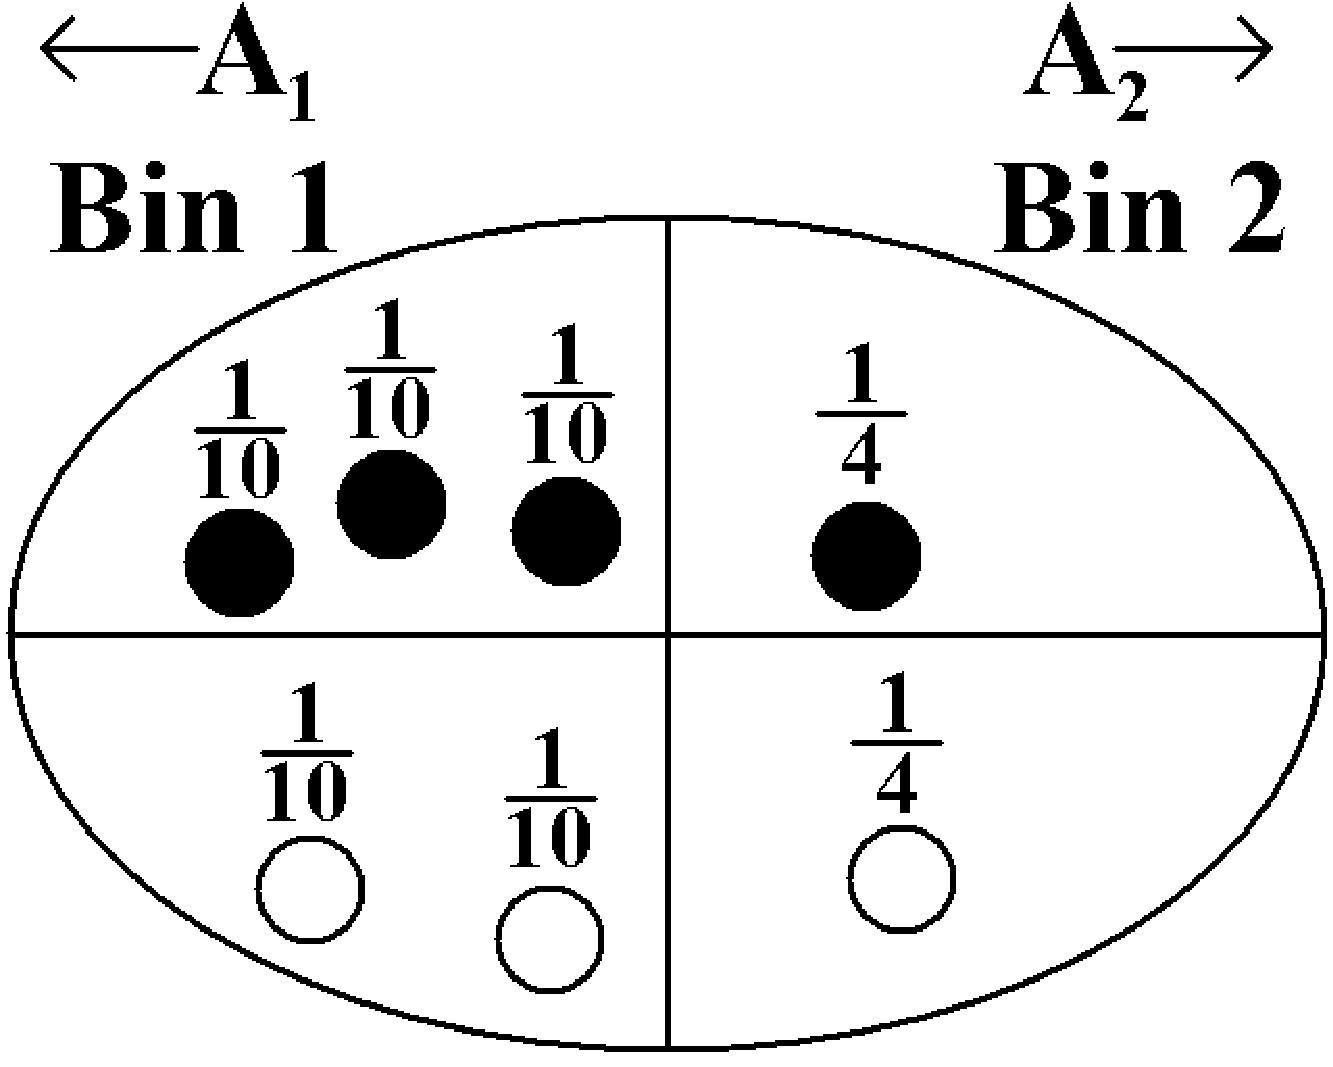
\includegraphics[bb = -500 0 0 520, scale = 0.24]{binprob.pdf}

This images shows that the sample space $\Omega$ is equal to the union of the events contained in bin 1($A_1$) and bin 2($A_2$), so $\Omega = A_1\cup A_2$. We can use the definition of conditional probability to see that

$\Pr[$Bin $1|$ \setlength{\unitlength}{.1in}
\begin{picture}(.5,1)(0,0)
\linethickness{1pt}
\put(-.25,.4){\circle{1}}
\end{picture}$] = \frac{\frac{1}{10} + \frac{1}{10}}{\frac{1}{10} + \frac{1}{10} + \frac{1}{4}}
 = \frac{\frac{2}{10}}{\frac{9}{20}} = \frac{4}{9}$
 
 Let us try to achieve this probability using Bayes' rule.  To apply Bayes' rule, we need to compute 
 $\Pr[ $ \setlength{\unitlength}{.1in}
\begin{picture}(.5,1)(0,0)
\linethickness{1pt}
\put(-.25,.4){\circle{1}}
\end{picture}$|$Bin $1]$, $\Pr[$Bin $1]$ and $\Pr[$ \setlength{\unitlength}{.1in}
\begin{picture}(.5,1)(0,0)
\linethickness{1pt}
\put(-.25,.4){\circle{1}}
\end{picture}$]$.  $\Pr[ $ \setlength{\unitlength}{.1in}
\begin{picture}(.5,1)(0,0)
\linethickness{1pt}
\put(-.25,.4){\circle{1}}
\end{picture}$|$Bin $1]$ is the chance that we pick a white ball given that we picked
bin 1, which is $\frac{2}{5}$. $\Pr[$ Bin $1]$ is $\frac{1}{2}$ as given in the description of the problem.
Finally, $\Pr[$ \setlength{\unitlength}{.1in}
\begin{picture}(.5,1)(0,0)
\linethickness{1pt}
\put(-.25,.4){\circle{1}}
\end{picture}$]$ can be computed using the Total Probability rule: 

$\Pr[$ \setlength{\unitlength}{.1in}
\begin{picture}(.5,1)(0,0)
\linethickness{1pt}
\put(-.25,.4){\circle{1}}
\end{picture}$] = \Pr[ $ \setlength{\unitlength}{.1in}
\begin{picture}(.5,1)(0,0)
\linethickness{1pt}
\put(-.25,.4){\circle{1}}
\end{picture}$|$Bin $1]\times\Pr[$Bin $1] + 
\Pr[ $ \setlength{\unitlength}{.1in}
\begin{picture}(.5,1)(0,0)
\linethickness{1pt}
\put(-.25,.4){\circle{1}}
\end{picture}$|$Bin $2] \times\Pr[$Bin $2] =  
\frac{2}{5}\times\frac{1}{2} + \frac{1}{2}\times\frac{1}{2} = \frac{9}{20}$. 
 
 Observe that we can apply the Total Probability rule here because
 $\Pr[$ Bin $1]$ is the complement of $\Pr[$ Bin $2]$. Finally, if we plug
 the above values into Bayes' rule we obtain the probability that
 we picked bin 1 given that we picked a white ball: 
 
 $\Pr[$Bin $1|$ \setlength{\unitlength}{.1in}
\begin{picture}(.5,1)(0,0)
\linethickness{1pt}
\put(-.25,.4){\circle{1}}
\end{picture}$] =
\frac{\frac{2}{5}\times\frac{1}{2}}{\frac{9}{20}}
= \frac{\frac{2}{10}}{\frac{9}{20}} = \frac{4}{9}$.

All we have done above is combined Bayes' rule and the Total Probability rule;
this is also how we obtained Equation (\ref{eq:update}). We could equivalently have
plugged in the appropriate values to Equation (\ref{eq:update}). 





\section*{Combinations of events}
In most applications of probability in Computer Science, we
are interested in things like $\Pr[\bigcup_{i=1}^n A_i]$
and $\Pr[\bigcap_{i=1}^n A_i]$, where the $A_i$ are simple
events (i.e., we know, or can easily compute, the $\Pr[A_i]$).
The intersection $\bigcap_{i} A_i$ corresponds to the logical
{\sc and} of the events~$A_i$, while the union $\bigcup_i A_i$
corresponds to their logical {\sc or}.  As an example, if $A_i$
denotes the event that a failure of type~$i$ happens in a certain
system, then $\bigcup_i A_i$ is the event that the system fails.

In general, computing the probabilities of such combinations
can be very difficult.  In this section, we discuss some
situations where it can be done. Let's start with independent events,
for which intersections are quite simple to compute. 

\subsection*{Independent Events}

\begin{definition}[Independence]
Two events $A,B$ in the same probability space
are \ul{independent} if $\Pr[A\cap B]=\Pr[A]\times \Pr[B]$.
\end{definition}

The intuition behind this definition is the following.  Suppose that
$\Pr[B]>0$.  Then we have  $$
   \Pr[A\vert B] = \frac{\Pr[A\cap B]}{\Pr[B]} = \frac{\Pr[A]\times \Pr[B]}{\Pr[B]} = \Pr[A]. $$
Thus independence has the natural meaning that ``the probability of~$A$ is not affected by
whether or not $B$ occurs.''  (By a symmetrical argument, we also have
$\Pr[B\vert A] = \Pr[B]$ provided $\Pr[A]>0$.)  For events $A,B$ such that
$\Pr[B]>0$, the condition $\Pr[A\vert B]=\Pr[A]$ is actually {\it equivalent\/}
to the definition of independence.

Several of our previously mentioned random experiments consist of independent events.
For example, if we flip a coin twice, the event of obtaining heads in the first trial
is independent to the event of obtaining heads in the second trial. The same applies
for two rolls of a die; the outcomes of each trial are independent. 

The above definition generalizes to any finite set of events:
\begin{definition}[Mutual independence]
Events $A_1,\ldots,A_n$ are \ul{mutually independent} if for every
subset $I\subseteq\{1,\ldots,n\}$, $$
   {\textstyle\Pr[\bigcap_{i\in I}A_i] = \prod_{i\in I}\Pr[A_i]}.  $$
\end{definition}

Note that we need this property to hold for {\it every\/} subset~$I$.

For mutually independent events $A_1,\ldots,A_n$, it is not hard to check
from the definition of conditional probability that,
for any $1\le i\le n$ and any subset $I\subseteq\{1,\ldots,n\}\setminus\{i\}$,
we have $$
     {\textstyle\Pr[A_i\vert \bigcap_{j\in I}A_j] = \Pr[A_i]}.  $$

Note that the independence of every pair of events (so-called {\it pairwise
independence\/}) does {\it not\/} necessarily imply mutual independence.
For example, it is possible to construct three events $A,B,C$ such that
each {\it pair\/} is independent but the triple $A,B,C$ is {\it not\/}
mutually independent.

\subsubsection*{Pairwise Independence Example}
Suppose you toss a fair coin twice and let $A$ be the event that the first flip is H's and
$B$ be the event that the second flip is H's. Now let $C$ be the event that both flips
are the same (i.e. both H's or both T's). Of course $A$ and $B$ are independent. 
What is more interesting is that so are $A$ and $C$: given that the first toss came up H's,
there is still an even chance that the second flip is the same as the first. Another way of 
saying this is that $P[A \cap C] = P[A]P[C] = 1/4$ since $A \cap C$ is the event that the 
first flip is H's and the second is also H's. By the same reasoning $B$ and $C$ are also
independent. On the other hand, $A$, $B$ and $C$ are not mutually independent. 
For example if we are given that $A$ and $B$ occurred then the probability that $C$ occurs
is $1$. So even though $A$, $B$ and $C$ are not mutually independent, every pair of them 
are independent. In other words, $A$, $B$ and $C$ are pairwise independent but not mutually 
independent. 

\subsection*{Intersections of events}
Computing intersections of independent events is easy; it follows from the definition. 
We simply multiply the probabilities of each event. How do we compute intersections
for events which may not be independent? From the definition of conditional probability, we immediately
have the following \ul{product rule} (sometimes also called the
\ul{chain rule}) for computing the probability
of an intersection of events.

\begin{theorem}[Product Rule] \label{thmpr}
For any events $A,B$, we have $$
   \Pr[A\cap B]= \Pr[A]\Pr[B\vert A].  $$
More generally, for any events $A_1,\ldots,A_n$, $$
   {\textstyle\Pr[\bigcap_{i=1}^n A_i] = \Pr[A_1]\times\Pr[A_2\vert A_1]\times
                                      \Pr[A_3\vert A_1\cap A_2]\times
                        \cdots\times\Pr[A_n\vert\bigcap_{i=1}^{n-1}A_i]}. $$
\end{theorem}

\begin{proof}
The first assertion follows directly from the definition of $\Pr[B\vert A]$
(and is in fact a special case of the second assertion with $n=2$).

To prove the second assertion, we will use induction on~$n$ (the number
of events).  The base case is $n=1$, and corresponds to the statement
that $\Pr[A]=\Pr[A]$, which is trivially true.  For the inductive step,
let $n>1$ and assume (the inductive hypothesis) that $$
   \Pr[{\textstyle\bigcap_{i=1}^{n-1} A_i}] = \Pr[A_1]\times\Pr[A_2\vert A_1]\times\cdots\times\Pr[A_{n-1}\vert{\textstyle\bigcap_{i=1}^{n-2} A_i}].  $$
Now we can apply the definition of conditional probability to the two
events $A_n$ and $\bigcap_{i=1}^{n-1} A_i$ to deduce that $$
\eqalign{\Pr[{\textstyle\bigcap_{i=1}^n A_i}] = \Pr[A_n\cap({\textstyle\bigcap_{i=1}^{n-1} A_i})]
                            &= \Pr[A_n\vert{\textstyle\bigcap_{i=1}^{n-1} A_i}]
                                      \times\Pr[{\textstyle\bigcap_{i=1}^{n-1} A_i}]\cr
                            &= \Pr[A_n\vert{\textstyle\bigcap_{i=1}^{n-1} A_i}]
                                      \times\Pr[A_1]\times\Pr[A_2\vert A_1]\times\cdots\times\Pr[A_{n-1}\vert{\textstyle\bigcap_{i=1}^{n-2} A_i}],\cr}  $$
where in the last line we have used the inductive hypothesis.
This completes the proof by induction.
\end{proof}

The product rule is particularly useful when we can view our sample
space as a sequence of choices.  The next few examples illustrate this
point.

\subsection*{Examples}

\subsubsection*{Coin tosses}  Toss a fair coin three times.  Let $A$ be
the event that all three tosses are heads.  Then $A=A_1\cap A_2\cap A_3$,
where $A_i$ is the event that the $i$th toss comes up heads.  We have $$
\eqalign{\Pr[A]&=\Pr[A_1]\times\Pr[A_2\vert A_1]\times\Pr[A_3\vert A_1\cap A_2]\cr
               &=\Pr[A_1]\times\Pr[A_2]\times\Pr[A_3]\cr
               &=\half\times\half\times\half={\textstyle{1\over 8}}.\cr}$$
The second line here follows from the fact that the tosses are
mutually independent. Of course, we already know that $\Pr[A]={1\over 8}$
from our definition of the probability space in the previous lecture note.
Another way of looking at this calculation is that it justifies our definition 
of the probability space, and shows that it was consistent with assuming that
the coin flips are mutually independent. 

If the coin is biased with heads probability~$p$, we get, again using
independence, $$
   \Pr[A] = \Pr[A_1]\times \Pr[A_2]\times \Pr[A_3] = p^3.  $$
And more generally, the probability of any sequence of $n$ tosses
containing $r$ heads and $n-r$ tails is $p^r(1-p)^{n-r}$.  This is
in fact the reason we defined the probability space this way
in the previous lecture note: we defined the sample point probabilities
so that the coin tosses would behave independently.


\subsubsection*{Monty Hall}
Recall the Monty Hall problem from the last lecture: there are three doors 
and the probability that the prize is behind any given door is $\frac{1}{3}$. There
are goats behind the other two doors. 
The contestant picks a door randomly, and the host opens one of the other two doors,
revealing a goat. How do we calculate intersections in this setting? For example, what is 
the probability that the contestant chooses door 1, the prize is behind door 2, and the host chooses
door 3? 

Let $A_1$ be the event that the contestant chooses door 1, let $A_2$
be the event that the prize is behind door 2, and let $A_3$ be the event
that the host chooses door 3. We would like to compute $\Pr[A_1\cap A_2\cap A_3]$. 
By the product rule:
$$
\Pr[A_1\cap A_2\cap A_3] = \Pr[A_1]\times \Pr[A_2|A_1] \times \Pr[A_3|A_1\cap A_2]
$$

The probability of $A_1$ is $\frac{1}{3}$, since the contestant is choosing the door at random.
The probability $A_2$ given $A_1$ is still $\frac{1}{3}$ since they are independent. The probability of the host choosing
door 3 given events $A_1$ and $A_2$ is 1; the host cannot choose door 1, since the contestant has already opened it, and
the host cannot choose door 2, since the host must reveal a goat (and not the prize). 
Therefore, 
$$
\Pr[A_1\cap A_2\cap A_3] = \frac{1}{3}\times\frac{1}{3}\times 1 = \frac{1}{9}.
$$

Observe that we did need conditional probability in this setting; had we simply multiplied
the probabilities of each event, we would have obtained $\frac{1}{27}$ since the probability of $A_3$
is also $\frac{1}{3}$ (can you figure out why?). What if we changed the situation, and instead asked for the probability
that the contestant chooses door 1, the prize is behind door 1, and the host chooses door 2? We can use the same technique as above,
but our final answer will be different. This is left as an exercise.

\subsubsection*{Poker Hands}
Let's use the product rule to compute the probability of a flush in a different
way. This is equal to $4\times\Pr[A]$, where $A$ is the
probability of a Hearts flush. Intuitively, this should be clear since there are 4 suits; we'll
see why this is formally true in the next section. We can write $A=\bigcap_{i=1}^5 A_i$,
where $A_i$ is the event that the $i$th card we pick is a Heart.
So we have $$
   {\textstyle\Pr[A]=\Pr[A_1]\times\Pr[A_2\vert A_1]\times\cdots\times
                \Pr[A_5\vert\bigcap_{i=1}^4 A_i]}.  $$
Clearly $\Pr[A_1]={{13}\over{52}}={1\over 4}$.  What about
$\Pr[A_2\vert A_1]$?  Well, since we are conditioning on~$A_1$ (the
first card is a Heart), there are only 51 remaining possibilities for
the second card, 12 of which are Hearts.
So $\Pr[A_2\vert A_1]={{12}\over{51}}$.  Similarly,
$\Pr[A_3\vert A_1\cap A_2]={{11}\over{50}}$, and so on.  So we get $$
   4\times\Pr[A]=4\times{{13}\over{52}}\times{{12}\over{51}}\times{{11}\over{50}}\times{{10}\over{49}}\times{{9}\over{48}},  $$
which is exactly the same fraction we computed in the previous lecture note.

So now we have two methods of computing probabilities in many of our
sample spaces.  It is useful to keep these different methods around,
both as a check on your answers and because in some cases one of the
methods is easier to use than the other.



\subsection*{Unions of Events}
You are in Las Vegas, and you spy a new game with the following rules.
You pick a number between 1 and~6.  Then three dice are thrown.  You
win if and only if your number comes up on at least one of the dice.

The casino claims that your odds of winning are 50\%, using the
following argument.  Let $A$ be the event that you win.  We can write
$A=A_1\cup A_2\cup A_3$, where $A_i$ is the event that your number
comes up on die~$i$.  Clearly $\Pr[A_i]={1\over 6}$ for each~$i$.
Therefore, $$
   \Pr[A]=\Pr[A_1\cup A_2\cup A_3] = \Pr[A_1]+\Pr[A_2]+\Pr[A_3]
                       = 3\times{1\over 6} = {1\over 2}.  $$
Is this calculation correct?  Well, suppose instead that the casino
rolled six dice, and again you win iff your number comes up at least
once.  Then the analogous calculation would say that you win
with probability $6\times{1\over 6}=1$, i.e., certainly!  The
situation becomes even more ridiculous when the number of dice gets
bigger than~6.

The problem is that the events $A_i$ are {\it not disjoint\/}: i.e.,
there are some sample points that lie in more than one of the~$A_i$.
(We could get really lucky and our number could come up on two
of the dice, or all three.)  So if we add up the $\Pr[A_i]$ we
are counting some sample points more than once.

Fortunately, there is a formula for this,
known as the \ul{Principle of Inclusion/Exclusion}:

\begin{theorem}[Inclusion/Exclusion]
For events $A_1,\ldots,A_n$ in some probability space, we have $$
   \Pr[{\textstyle\bigcup_{i=1}^n A_i}] = \sum_{i=1}^n \Pr[A_i]
                             -\sum_{\{i,j\}} \Pr[A_i\cap A_j]
                             +\sum_{\{i,j,k\}} \Pr[A_i\cap A_j\cap A_k]
                             -\cdots\pm \Pr[{\textstyle\bigcap_{i=1}^n A_i}].  $$
[In the above summations, $\{i,j\}$ denotes all unordered pairs
with $i\ne j$, $\{i,j,k\}$ denotes all unordered triples of distinct
elements, and so on.]
\end{theorem}

I.e., to compute $\Pr[\bigcup_i A_i]$, we start by summing the event
probabilities $\Pr[A_i]$, then we {\it subtract\/} the probabilities
of all pairwise intersections, then we {\it add\/} back in the probabilities
of all three-way intersections, and so on.

We won't prove this formula here; but you might like to verify it
for the special case $n=3$ by drawing a Venn diagram and checking
that every sample point in $A_1\cup A_2\cup A_3$ is counted exactly
once by the formula.  You might also like to prove the formula for
general~$n$ by induction (in similar fashion to the proof of the Product
Rule above).

Taking the formula on faith, what is the
probability we get lucky in the new game in Vegas?  $$
  \Pr[A_1\cup A_2\cup A_3] = \Pr[A_1]+\Pr[A_2]+\Pr[A_3]
                  -\Pr[A_1\cap A_2] -\Pr[A_1\cap A_3] -\Pr[A_2\cap A_3]
                                +\Pr[A_1\cap A_2\cap A_3].  $$
Now the nice thing here is that the events $A_i$ are mutually
independent (the outcome of any die does not depend on that of the
others), so $\Pr[A_i\cap A_j]=\Pr[A_i]\Pr[A_j] = ({1\over 6})^2={1\over{36}}$,
and similarly $\Pr[A_1\cap A_2\cap A_3]=({1\over 6})^3={1\over{216}}$.
So we get $$
  \Pr[A_1\cup A_2\cup A_3] = {\textstyle \left(3\times{1\over 6}\right) -
                                         \left(3\times{1\over {36}}\right) +
                                         {1\over{216}} =
                                             {{91}\over{216}}\approx 0.42}. $$
So your odds are quite a bit worse than the casino is claiming!

When $n$ is large (i.e., we are interested in the union of many events),
the Inclusion/Exclusion formula is essentially useless because it
involves computing the probability of the intersection of every non-empty
subset of the events: and there are $2^n-1$ of these!  Sometimes
we can just look at the first few terms of it and forget the rest:
note that successive terms actually give us an overestimate and then
an underestimate of the answer, and these estimates both get better
as we go along.

However, in many situations we can get a long way by just looking at
the \ul{first} term:
\begin{enumerate}
\item {\bf Disjoint events.}  If the events $A_i$ are all {\it disjoint\/}
(i.e., no pair of them contain a common sample point --- such events
are also called {\it mutually exclusive\/}), then $$
   \Pr[{\textstyle\bigcup_{i=1}^n A_i}] = \sum_{i=1}^n \Pr[A_i].  $$
[Note that we have already used this fact several times in our examples,
e.g., in claiming that the probability of a flush is four times the
probability of a Hearts flush --- clearly flushes in different
suits are disjoint events.]
\item {\bf Union bound.}  Always, it is the case that $$
   \Pr[{\textstyle\bigcup_{i=1}^n A_i}] \le \sum_{i=1}^n \Pr[A_i].  $$
This merely says that adding up the $\Pr[A_i]$ can only {\it over\/}estimate
the probability of the union.  Crude as it may seem,
in the next lecture note we'll see how to use the union bound effectively
in a Computer Science example.
\end{enumerate}
\end{document}
